\chapter{Theoretical background}
\section{Phonetics and phonology}\label{sec:2.1}
When speakers produce speech, they modify their larynx and vocal organs in a particular way, shaping the cavities through which air passes. This results in specific patterns of disturbance to the air-molecules that spread outwards and eventually reach the ear of the listener where they are processed by the auditory system. For example, bilabial stops are common sounds in human languages. They are characterised by a complete closure of the lips, during which air cannot escape through the oral tract and intra-oral pressure builds up. When the closure is released, the compressed air escapes in a characteristic burst. Both the closure interval and the release phase create a certain disturbance to the air molecules. The resulting subtle differences in air pressure variation can then be detected by the human ear.

For a complete scientific assessment of human speech, these physical and biological mechanisms must be investigated. At the same time, humans use these mechanisms in a very particular way. Speakers classify objectively different instances of articulatory / acoustic / auditory events. The resulting categories can further be described to have a certain functional value for the communicative system. This allows the listener to perceive two observations differing in a particular physical dimension as two instances of the same category. At the same time, another two observations exhibiting the same difference in a different context may be perceived as two different categories. Take for example voice onset time (VOT). VOT is defined as the interval between the release of an oral stop consonant and the onset of voicing. It is a parameter that can vary continuously. However, many languages exhibit systematic clusters of VOT values corresponding to different sets of words. For example, in English\il{English}, syllable-initial stops in words like \textit{bear} have been reported to exhibit VOT values around 0 ms, i.e. the voicing starts with the release of the stop. Syllable-initial stops in words like \textit{pear} have been reported to exhibit positive VOT values around 60 ms (e.g. \citealt{LiskerAbramson1964}). Within a particular part of the continuum, VOT values differing within a certain range are interpreted as belonging to the same category. However, the same absolute difference in VOT values elsewhere on the continuum may reflect instances of two different categories (e.g. \citealt{Liberman.etal1957}). 

Thus, understanding speech not only involves comprehensive models of the physical and biological prerequisites of speech, but also involves understanding of how speakers categorise speech phenomena, form functional categories, and how these categories interact with each other within a system. These two sides of the coin are traditionally attributed to the linguistic subfields of ‘phonetics’ and ‘phonology’, respectively. Phonetics can be conceived of as the assessment of speech sounds from an objective perspective based on physical and biological observations. Phonology can be conceived of as the assessment of speech sounds from an internal perspective, analysing the functional relevance of them in relation to other elements within the same system. 

For the latter, phonology, we can distinguish between two traditions. These traditions differ with respect to the methodologies applied as well as the assumed scope of phonological analysis. Note that, for  exposition purposes, the following discussion simplifies the diversity of phonological schools. The scientific landscape is, of course, more complex. 

On the one hand, there is a tradition that we will refer to as ‘theoretical phonology’, which is based on linguistic structuralism (\citealt{Sapir1925,Bloomfield1933,Trubeckoj1939,Saussure1989}). In this tradition, phonological units are considered as functional elements that have to be defined by their functions within the language system (e.g. \citealt{Trubeckoj1939}). Functional elements are represented as symbols, i.e. they are represented as symbolic abstractions of their actual physical manifestation. This systemic approach later led to the development of phonological analyses that are theoretical in nature. Similar to theoretical physics, structures and principles are proposed that account for the observations, regardless of whether they are observable themselves (\citealt{Gussenhoven2015}). An example is the concept of allophony. Two phonetically distinct speech segments can be considered contextual variants of an underlying phoneme (if these variants are in complementary distribution and sufficiently similar). Take for example voiceless oral stops in syllable-initial sibilant clusters in English, like in the word \textit{sport}. These stops are characterised by VOT values around 0 ms. As discussed above, corresponding voiceless bilabial stops in absolute syllable-initial position (e.g. \textit{pear}) are usually characterised by VOT values around 60 ms. Despite these two sounds being physically distinct, they are commonly analysed as allophones of one underlying phoneme (/p/). Thus, the phoneme /p/ is assumed to have contextual variants, one with aspiration (long VOT, [pʰ]) and one without aspiration (zero VOT, [p]). While the phoneme itself cannot be observed or measured directly, since it is an abstract notion, it can be considered a relevant concept to describe distributional observations of the English sound system in a parsimonious way. The tradition of theoretical phonology focuses on contrasting features of a sound system. This allows for a description of a sound system by proposing a small inventory of symbols and a finite set of interactions between these symbols. This type of phonological analysis is an important prerequisite for the academic communication of critical properties of a sound system, enables language teaching, and allows a straightforward cross-linguistic comparison of sound systems.\il{English} 

Alternatively, phonology can also be conceived of as the scientific study of the cognitive underpinnings of sound patterns. Such a cognitive understanding of speech was most prominently formulated by \citet{ChomskyHalle1968} who stated their primary interest in the “competence” of a speaker. Competence refers to the knowledge of “the grammar that determines an intrinsic connection of sound and meaning for each sentence” (\citealt[3]{ChomskyHalle1968}). Although many phonologists have moved past the ideas of generative phonology, a focus on cognitive aspects of speech has since then dominated phonological analysis. It is most prominently defined by the ‘Laboratory Phonology’ movement (e.g. \citealt{Pierr.etal2000}), according to which language is conceived of as a phenomenon of nature. In that vein, language has to be explained in terms of general facts about the physical world, biological and cognitive capabilities of humans, and their interaction with the environment. Rapid technological advancements have led to a multitude of methods enabling the investigations of cognitive representations that underlie speech communication. The physical aspects of speech are studied in the context of memory formation, categorisation, as well as the cognitive development of categories during language acquisition. 

While a descriptive formalisation of a sound system in the tradition of theoretical linguistics may be taken as a departure point for hypotheses about linguistic knowledge, the former should not be confused with the latter. It is necessary to distinguish between these two definitions of the scientific object explicitly. Traditional phonological descriptions are formalisations of phonetic observations within an abstract symbol system, mainly disregarding non-contrastive phonetic information. As opposed to that, a large body of research has argued that the cognitive representation of speakers is less abstract, but rather contains a large amount of non-contrastive information (among many others \citealt{Goldinger1998,Hawkins2003}; and see \citealt{Hawkins2012} and \citealt{Pierr2012} for overviews).

This book will explore certain phonetic aspects of stress and intonation in Tashlhiyt that convey contrastive meaning. Based on quantitative observations, we will propose an abstract description of the phonetic facts in the tradition of structuralism and theoretical phonology. These abstract formalisms serve descriptive purposes and allow for cross-linguistic comparison, but their use should not be interpreted as capturing how the actual knowledge of a speaker is represented. For the purpose of formalisation,\footnote{Of course, this does not exclude the possibility that proposed phonological formalisms are adequate departure points for further psycholinguistic modelling.} we choose the Autosegmental-Metrical model. This model is introduced in subsequent sections alongside relevant concepts and terminology of intonation theory that will be used to describe stress and the placement of intonational tones in Tashlhiyt.

First, the two broadly used notions ‘intonation’ and ‘prosodic structure’ will be introduced and distinguished (\sectref{sec:2.2}). Subsequently, the mapping between tonal events and prosodic structure will be discussed with regard to two descriptive categories: ‘edge tones’ and ‘pitch accents’ (\sectref{sec:2.3}). Edge Tones are tonal events that are associated to the edges of prosodic constituents. Pitch accents are tonal events that are associated to specific prosodic units, so-called ‘tone bearing units’ (TBU). In some cases, the available TBUs are insufficient to carry pitch movements, i.e. there is not enough segmental material available to realise the pitch movement, or the segmental material is phonetically not suited to bear a pitch movement. Intonation systems allow for different adjustments of the segmental tier or the tonal tier in order to accommodate such conflicts. The nature of these adjustments is controversial. They can either be considered to be adjustments of the phonetic realisation of tonal contours or reflexes of phonological differences. The different adjustments as well as their theoretical treatment is discussed to prepare the investigation of tonal placement patterns in Tashlhiyt in later chapters (\sectref{sec:2.4}). \is{edge tone}\is{pitch accent}\is{boundary}\is{tone bearing unit}


\section{Suprasegmental phonology}\label{sec:2.2}
 
Phenomena that refer to domains larger than segments (phones/phonemes), such as the syllable, the word or entire phrases, are referred to as ‘suprasegmental’. Postlexical suprasegmental properties of speech encode phenomena that are not lexically determined but dependent on the postlexical structure of the discourse. These aspects of speech not only encode paralinguistic functions, such as emotions, speaker involvement, and attitude; they also play a crucial role in linguistic organisation. Their central role has been tremendously under-represented in linguistic research in the 20th century leaving the majority of documented languages, in fact, under-documented with regard to their suprasegmental phonological system. The language investigated in this book is a good example of this lack of documentation. \is{paralinguistic}

Yet, anyone who has tried to communicate a relevant message with a mouth full of food (“can you pass me the gravy, please.”) is likely aware of the immense role that suprasegmental properties of speech play when the actual segments are unintelligible. Suprasegmental parameters convey the intended illocutionary act, structure the utterance into smaller meaningful units, and emphasise certain units while de-emphasising less important pieces of information. The entire discourse, including turn-taking between interlocutors, is controlled by suprasegmental aspects of speech. When we talk about suprasegmental properties of linguistic structure, two terms are often used interchangeably: intonation and prosodic structure. In the following, we attempt to arrive at working definitions for these terms within the terminology and conceptual framework of the ‘Autosegmental-Metrical’ model, henceforth referred to as AM model (\citealt{Pierr1980}; see \citealt{Ladd2008} for an overview).

The reason for using the AM model are twofold: first, it is the most commonly used model to describe intonation systems. Thus, many languages that have already been documented with regard to prosodic and intonational structure are described within this analytical framework. In this respect, AM has proved to be flexible enough to adapt to the analytical requirements of typologically diverse languages. There is of course a high degree of variability as to how the model is interpreted and applied to the language under investigation by a given analyst. The basic descriptive devices it offers, however, allow one to compare languages reasonably well. Second, the AM model captures common properties of prosodic and intonational systems, which explains the great success this model had after its initial development in the 1980’s.

The ‘Autosegmental’ aspect of AM is based on the assumption that there are separate levels of description for segments on the one hand (i.e. consonants and vowels) and tonal events on the other hand. The ‘Metrical’ aspect of AM is based on the assumption that elements within the segmental levels of description are incorporated into hierarchically organised sets of constituents. These assumptions are discussed in detail below. 

In the AM model, the terms ‘prosodic structure’ and ‘intonation’ are defined in a narrow sense (\citealt{Grice2006,Ladd2008}). Prosodic structure is the system that groups utterances into smaller units and assigns relative prominence to elements within these units. Intonation is the system that associates tonal events with this prosodic structure. 

\newpage 
Prosodic structure and intonation are phonetically manifested in a multitude of different channels including perceived pitch (acoustically approximated by fundamental frequency), loudness (relative intensity), vowel quality (formant bandwidth, spectral tilt, voice source), and length of certain units (relative duration). Consider for example the following English sentences:\il{English}

\begin{exe}
\ex\label{ex:2:1}   Helen LOVES cheese. 
\ex\label{ex:2:2}   Helen  loves cheese straws.
\end{exe}

For example, the word \textit{loves} in \REF{ex:2:1} can be made prominent by realising a rise in pitch, accompanied by longer, louder, and more clearly articulated segments, than it would otherwise be. Similarly, the word \textit{cheese} can be marked as phrase final in \REF{ex:2:1} as opposed to \REF{ex:2:2} where it is phrase medial. Finality in \REF{ex:2:1} can be marked by a fall in pitch on \textit{cheese} accompanied by creaky voice, a decrease in loudness, and lengthening of its final segments. 

\subsection{Prosodic structure}
The AM model assumes that utterances can be broken down into prosodic units that are hierarchically organised. Although certain prosodic units have been claimed to be found in all languages, their universality has been called into question. Moreover, the validity of such claims is very much dependent on how the units are defined (e.g. \citealt{Schiering.etal2010,Hyman2011}). Cross-linguistically, some prosodic units are found to be more common than others, such as the following: the highest level in the hierarchy is commonly referred to as either the ‘utterance’ (υ) or the ‘intonational phrases’ (“ı” or “IP”) which itself can contain one or more ‘smaller phrases’ (here referred to as “SP”). Depending on the analysis, either there are no levels between the intonation phrase and the phonological word, the next level in the hierarchy, or there are one or more levels. These levels have been referred to as phonological phrases (“φ” or “PP”, e.g. \citealt{Gussenhoven2004}, for English), accentual phrases (“α” or “AP”, e.g. \citealt{PierrBeck1988}, for Japanese) or intermediate phrases (“ip”, e.g.  \citealt{BeckmanPierr1986}, for English; and \citealt{Grice.etal2005ger}, for German). Regardless of how it is labelled, any SP is assumed to contain one or more phonological words (“ω”). Words might be organised into metrical feet (“∑” or “F”) which themselves are organised into one or more syllables (“σ”). Syllables can be further organised into subsyllabic constituents subsuming the segments (‘onset’ and ‘rhyme’, the latter of which can be further decomposed into ‘nucleus’ and ‘coda’). Alternatively, some accounts propose the mora (“μ”), which divides the syllable into rhythmic units. An example hierarchy of prosodic units in English is shown in \figref{fig:2.1}.\il{English}\il{Japanese}\il{German}

\begin{figure}
  \centering 
   
\includegraphics[width=0.8\textwidth]{figures/Figure_2_1.png}
  \caption{Schematised example of a hierarchically organised prosodic structure for the English sentence “Too many cooks spoil the broth”. At the bottom, the tonal structure is represented in accordance with Beckman and Pierrehumbert’s analysis of English (\citeyear{BeckmanPierr1986}). See \citet{Gussenhoven2002} for an alternative analysis. This example has been presented by ibid. (2002:271).}
   \label{fig:2.1}
   \end{figure}

The proposed level of prosodic structure can be justified by distributional diagnostics. For example, in English,\il{English} the IP and the ip have been defined intonationally (\citealt{BeckmanPierr1986}), i.e. certain tonal events appear at their edges. For instance, a rise in pitch, may only occur at the right (or left) edge of the proposed prosodic unit. So in \figref{fig:2.1}, there is a high edge tone at the right edge of the initial ip (notated with ‘-’, i.e. H-) and a low edge tone at the right edge of the final ip (L- coinciding with the right edge of the IP, notated with ‘\%’, i.e. L\%). Other phonetic aspects can be taken to back up this descriptive choice. In addition to the presence of the tonal event, there can be a clear pause after the proposed unit. Further evidence is sought in modifications of segmental properties. First, specific segmental processes such as assimilations have been argued to operate only within certain prosodic phrases but not across their edges (\citealt{NesporVogel1986}). Second, it has been repeatedly shown that fine phonetic detail is used to encode prosodically privileged positions, such as edges of prosodic domains. This segmental marking of prosodic structure is henceforth referred to as ‘edge-induced strengthening’. Edge-induced strengthening comprises the modification of temporal and spatial phonetic parameters of prosodic phrases. Many languages have been shown to mark certain prosodic edges by phonetically enhancing segments either before or after the boundary. There are two major phenomena described in the literature that fall under the umbrella of edge-induced strengthening: ‘initial strengthening’ and ‘final lengthening’. The former refers to spatio-temporal adjustments at the left edge. For example, it has been shown that acoustic parameters that are contrastive are enhanced in phrase-initial position. For instance, in languages that have aspirated stops, voice onset time (VOT) is longer in phrase-initial position than in phrase-medial position (\citealt{Cooper1991,PierrTalkin1992,Jun1993,ChoSun2000,Choi2003,Cole.etal2003}). The latter, final lengthening, refers to the spatio-temporal adjustment of segments at the right edge of a phrase. For example, it has been shown that the syllable rhyme is longer in phrase-final position than in phrase-medial position in English \il{English} (e.g. 
\citealt{TurkShattuck2007}). \is{edge tone}

The proposed hierarchically organised prosodic units involve strength relationships. This concept is borrowed from the tradition of ‘Metrical Phonology’ (\citealt{Leben1976,LibermanPrince1977}). To demonstrate this idea, consider the compound \textit{statistics instructor} (cf. \figref{fig:2.2}). The compound consists of two prosodic elements corresponding to the nouns \textit{statistics} and \textit{instructor}. Both words consist of three syllables. One syllable of each word is considered to be the metrically strongest syllable, i.e. the stressed syllable (/stə.ˈtɪs.tɪks/ and /in.ˈstrʌk.tə/). Strength relations are phonetically manifested via parameters such as duration and intensity (see Chapter 4 for a detailed discussion). In addition to the strength relation within each noun, there is a strength relation on the level of the whole compound. The first part of the compound is stronger than the second part.\footnote{For exposition purposes, we ignore the level of the metrical foot here.}

\begin{figure}
  \centering 
   
\includegraphics[width=0.5\textwidth]{figures/Figure_2_2.png}
  \caption{Schematised example of strength relationships in the compound \textit{statistics instructor}. The two parts of the compound have at least one strong syllable and the compound itself is characterised by a strong first element and a weak second element}
   \label{fig:2.2}
   \end{figure}


This hierarchy of strength relations results in one single most prominent syllable of the whole compound. It is the strong syllable of the strong noun (/ˈtɪs/). This is reflected in the perception of that syllable as the most prominent syllable of the compound overall. The strongest element of a unit is called the ‘designated terminal element’ (\citealt{LibermanPrince1977,Ladd2008}). It is the docking site for particular tonal movements, linguistically significant parts of the intonation contour. 

\subsection{Intonation}
In the AM model, prosodic structure is taken as a grid that determines where significant aspects of the intonation contour may occur. Of the phonetic dimensions described above, pitch has been regarded as the primary channel of intonation as defined here. Acoustically, pitch corresponds roughly to the perception of fundamental frequency (f0). Changes in pitch, such as a pitch glide or jump up or down from the pitch of surrounding segmental material, are perceptually most prominent. These changes in pitch often co-occur systematically with a particular pragmatic or semantic function and are therefore considered to be phonological units formally integrated into the phonological system as abstract entities.

Tonal movements can be conceptualised as configurations, i.e. holistic contours that directly reflect functional aspects of speech (e.g. \citealt{Bolinger1951,Crystal1969,Halliday1967,OConnorArnold1973,Kohler1991,HirstDiCristo1998,Xu2005}). Alternatively, tonal movements can be considered to consist of sequences of tonal targets. These are compositional in that the function of the whole utterance can be deduced from the functions of its parts. The latter approach assumes that tonal structure consists of a sequence of local tonal targets and that the pitch values between such tonal targets are phonologically underspecified, i.e. they are merely transitions from one target to the next. These tonal targets are formally represented as either H(igh) or L(ow) tones and are assumed to systematically co-occur with certain structural landmarks. Commonly, tones co-occur with prominent elements of the prosodic structure and / or edges of prosodic constituents.

Configurational approaches have been criticised due to their inability to account for certain characteristics of intonational contours. If intonational contours were holistic undivided forms, one would expect them to stretch or compress according to the length of the utterance (\citealt{Arvaniti2011}). This is, however, not the case. \figref{fig:2.3} depicts an intonational contour that has been prominently discussed by Hirschberg and Ward (\citealt{WardHirsch1985,HirschbergWard1992}). 

\begin{figure}
  \centering 
   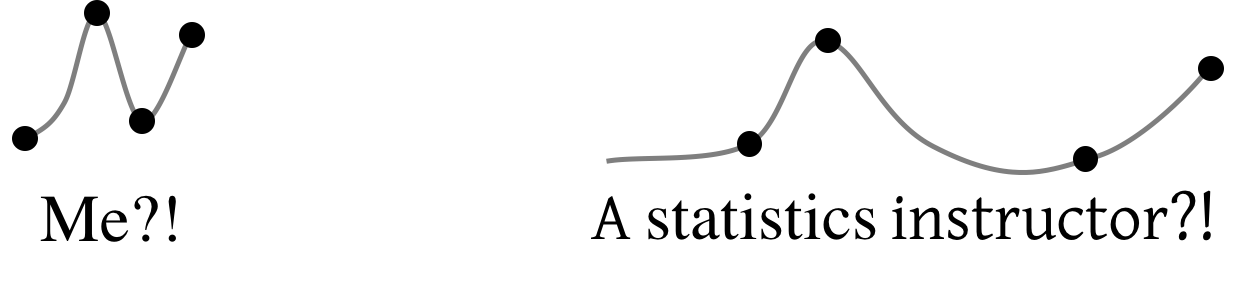
\includegraphics[width=0.8\textwidth]{figures/Figure_2_3.png}
  \caption{Schematic depiction of the ‘incredulity contour’ (\citealt{HirschbergWard1992,Ladd2008,Arvaniti2011})}
   \label{fig:2.3}
   \end{figure}
   
This contour is described as being used to express a “lack of speaker commitment” to the appropriateness of a proposition in general (\citealt[243]{HirschbergWard1992}). \il{English}More specifically, it is used to express incredulity. Imagine a scenario in which my supervisor approaches me and suggests that I give a course in statistics next semester. At this particular point in time, I may consider myself still very poorly educated within the depths of statistical thinking and do not feel suited for this assignment. My surprise and incredulity would potentially be expressed by the contour depicted in \figref{fig:2.3} (in the very rare occasion in which I used native English intonation contours appropriately).

This contour can be holistically described as a rise-fall-rise. If this were an appropriate description of the contour expressing the proposed function, we would expect it to be evenly distributed across the segments, when comparing the short utterance \textit{Me?!} with the longer utterance \textit{A statistics instructor?!}. The contour on \textit{Me?!} is, however, not simply stretched to fit the longer utterance. There are at least two separate tonal events: the rise and subsequent fall through the prominent lexically stressed syllable (here: stə.ˈtɪs.tɪks) and the utterance-final rise. These tonal events are matched with certain very specific structural landmarks. Between these tonal events, there is a long stretch of low pitch dependent on the length of the utterance. This is in line with evidence that intonational contours differ in their alignment in utterances of varying length, prosodic structure, and information structure. This was first instrumentally recognised by proponents of the Institute for Perception Research model in Eindhoven (IPO, \citealt{CohenHart1968,HartCohen1973,HartCollier1975}). They found that in Dutch \il{Dutch}a sequence of pitch movements is realised on specific landmarks in the utterance. These landmarks are sometimes realised on one syllable and are sometimes realised on two non-adjacent syllables separated by a longer stretch of segments. Subsequent research on unrelated languages supported the observation that certain aspects of the contour timed with certain landmarks of the prosodic structure are important for listeners, but overall contour shape is not. For instance, \citet{PierrSteele1989} recreated an artificial contour for the expression \textit{only a millionaire} that can be described as a rise-fall followed by a rise utterance finally. They created a continuum consisting of 15 positions for the rise-fall differing by 20 ms. Speakers interpreted the continuum as two different contours: one contour with an early aligned rise-fall and one with a late aligned rise-fall. These two different contours correspond to two different pragmatic interpretations. This demonstrates that certain tonal events systematically co-occur with very specific landmarks of the prosodic structure. Similar observations have been made by \citet{RietveldGussenhoven1995} for Dutch\il{Dutch}, and \citet{DimperioHouse1997} for Neapolitan Italian\il{Italian (Neapolitan)}. Contours with the same overall shape are interpreted as different communicative functions dependent on the temporal co-occurrence of certain tonal events with certain structural landmarks.

Configurational approaches cannot capture the systematic co-occurrence of parts of the contour and certain structural landmarks in the utterance. It is necessary to decompose the contour into separate parts, which are located in specified positions of the utterance. This allows the analyst to model the differences between intonation contours associated with different functions successfully, and allows, at the same time, to capture the shared structure of superficially different looking contours expressing the same function. This requires a level of abstraction that is achieved in the AM model by decomposing the intonation contour into separate tonal events that are associated to particular prosodic positions.
   
\section{Tonal events}\label{sec:2.3}
In the AM model, a tonal event can either co-occur with a tone bearing unit of a prosodic constituent (TBU) or co-occur with the periphery of a constituent itself. The co-occurrence of a phonological tone with a certain segmental or prosodic landmark can be expressed in terms of ‘phonological association’ and ‘phonetic alignment’. Henceforth, association is taken to be discrete, referring to the phonological linking of a tone with a phonological entity (a TBU or a boundary), and alignment to be continuous, referring to the exact position of a tone in relation to a landmark in the speech signal (see e.g. \citealt{Ladd2008}). The former is an abstraction away from the phonetic instantiation captured by the latter. The mapping of a tonal event (tune) onto the segments it co-occurs with (text) is referred to as ‘tune-text-association’.\is{tone bearing unit}\is{tonal association}\is{tonal alignment}

There is a crucial distinction between edge tones, i.e. tones found at the beginning or end of a prosodic constituent, and pitch accents, i.e. tones marking strong elements of prosodic constituents. This distinction is made in the AM model, as well as in some models preceding it. \citet{Trubeckoj1939} distinguished between tones having a ‘culminative’ and a ‘delimitative’ function. Culminative tones lend prominence; delimitative tones mark edges. \citet{TragerSmith1951} made a distinction between ‘pitch phonemes’ and ‘juncture phonemes’. The IPO model distinguished between ‘accent lending’ and ‘non-accent-lending’ pitch movements (\citealt{CohenHart1968,HartCohen1973,HartCollier1975}). In the AM model, this distinction is made using the terms ‘edge tones’ and ‘pitch accents’. Generally, these two types of tonal events are widely used descriptive categories that capture tonal events in intonation systems across languages.\is{edge tone}\is{pitch accent}

\subsection{Edge tones}
Tonal events can co-occur with the beginning or end of a prosodic constituent. These tones are called ‘edge tones’ or ‘boundary tones’. Edge tones mark edges but also express utterance-wide functions such as sentence modality. In the incredulity contour shown in \figref{fig:2.3}, the final rise always occurs at the right edge of the phrase. It has been analysed as a H(igh) intonation phrase-final edge tone (\citealt{HirschbergWard1992}). In \figref{fig:2.1}, the right boundary of the first ip is marked by a high edge tone marking non-finality (H-), while the final ip is marked by a low edge tone (L-). Ladd defines edge tones as “any tone that is associated with the periphery of a prosodic domain” (\citealt[47]{Ladd2008}). This phonological association is often manifested as the tone being aligned close to the edge of the phrase. This is made explicit by \citet[127]{PierrBeck1988}: they claim that “tones are produced at the phonetic boundary of the node with which they are associated […].” They go on and state that “the initial and final tone […] are produced at about the same time as the initial and final segments […]”. Thus, the most relevant characteristic of an edge tone is its alignment with the margins of a prosodic phrase.\is{edge tone}\is{tonal association}\is{tonal alignment}

\subsection{Pitch accents}
After having explored the properties of tones that are located at the periphery of prosodic phrases, we now turn to tones that occur with prominent units inside these phrases. Pitch accents have been described as marking the strongest elements (or the heads) of prosodic constituents.\footnote{Please note, that the term ‘pitch accent’ has also been used to refer to lexically determined tonal properties of certain languages, most prominently used in the description of Japanese. The term is used here only to refer to post-lexical pitch accents.}\is{pitch accent}

In English and German for example, a pitch accent is usually associated with the primary stressed syllable of the most prominent word of a phrase. Going back to the short incredulity contour in \figref{fig:2.3}, the rise-fall in pitch has been described as a rising pitch accent, associated with the primary stressed syllable of \textit{statistics instructor}. The pitch accent that co-occurs with the stressed syllable of the most prominent unit of a phrase is commonly described as the nuclear pitch accent of that phrase. Commonly the nuclear pitch accent occurs within focused constituents, i.e. communicatively the most relevant elements of the utterance (for a brief discussion of ‘focus’, see Chapter 5). The concept of marking the head of a constituent is directly linked to the idea of strength relationships within the prosodic structure and is determined, among other things, by lexical strength relationships within the word.\is{pitch accent}\is{focus}\il{English}\il{German} 

\section{Tune-text-association}\label{sec:2.4}
The previous discussion highlighted two descriptive categories of tonal events in the AM model: edge tones and pitch accents. These tones are mainly distinguished by their temporal co-occurrence with certain segmental landmarks. An edge tone is aligned with the edge of a phrase and a pitch accent is aligned with the head of a phrase. Phonetic alignment is taken as direct evidence for any proposed phonological association (\citealt{Arvaniti.etal2000}). Proposing the association of a tone to an edge is often justified by the consistent alignment of the tone to that edge. Proposing the association of a tone to a TBU is justified by the consistent alignment of the tone to that TBU.\is{pitch accent}\is{edge tone}\is{tonal alignment}\is{tonal association}\is{tone bearing unit}

The last two decades of research investigating phonetic alignment have yielded the insight that certain tonal targets can be aligned in a highly systematic way with respect to reference points in the segmental string. In a number of European languages, specific turning points (local F0 minima and F0 maxima as well as elbows) are predictably realised within a small time frame determined by the segmental make-up of the text (e.g. \citealt{Arvaniti.etal1998,AttererLadd2004,ArvanitiLadd2009,Muecke.etal2009}, and \citealt{Ladd2008} for an overview). Importantly, patterns of phonetic alignment relative to segments, which are consistent within rather than across language varieties, are typically taken as the phonetic manifestation of phonological association to a structural unit like a stressed syllable or a phrase edge (\citealt{Arvaniti.etal2000}). This, in turn, goes hand in hand with a classification of the tonal event as belonging to a descriptive category like pitch accent or edge tone.\is{pitch accent}\is{edge tone}\is{tonal alignment}\is{tonal association}

Similarly, the existence of varying alignment patterns where the same tonal targets are aligned differently relative to a stressed syllable has frequently been used to posit a distinction between pitch accent categories within a language variety (\citealt{PierrSteele1989,DimperioHouse1997,FacePrieto2007}), which we will turn to now.\is{pitch accent}\is{tonal alignment}

In the AM model, pitch accents are analysed as consisting of minimally one tone which is ‘starred’ (e.g. H*, L*). The starred tone can optionally be combined with an ‘unstarred’ tone (e.g. H*+L, L+H*, signalled by ‘+’, but see \citealt{Gussenhoven2002}, for a critique of this notation). In those bitonal cases, one common argument for choosing which tone is the starred tone and which is the unstarred tone relates to the phonetic alignment of the starred tone with respect to the segmental material. \figref{fig:2.4} depicts two different pitch accent types for English\il{English}. Both involve a rise in pitch close to the TBU, the stressed syllable (grey box), but they differ in terms of phonetic alignment. The solid line corresponds to a rise starting within the stressed syllable and reaching its pitch maximum in the following syllable. The dashed line corresponds to a rise starting in the syllable preceding the stressed syllable and reaching its pitch maximum within the stressed syllable. This difference in phonetic alignment can be accounted for by means of the notation of the starred tone, which indicates which tonal target is reached in the stressed syllable.\footnote{The notation of starred tones is not uncontroversial since it often remains empirically unclear which tone of a bitonal event is the starred one (\citealt{Arvaniti.etal2000}). Moreover, it often remains a matter of analysis whether the unstarred tone of a bitonal event really ‘belongs’ to the pitch accent or whether it might be a reflex of a preceding/following pitch accent or an edge tone.}\is{pitch accent}\is{tonal alignment}

\begin{figure}
  \centering 
   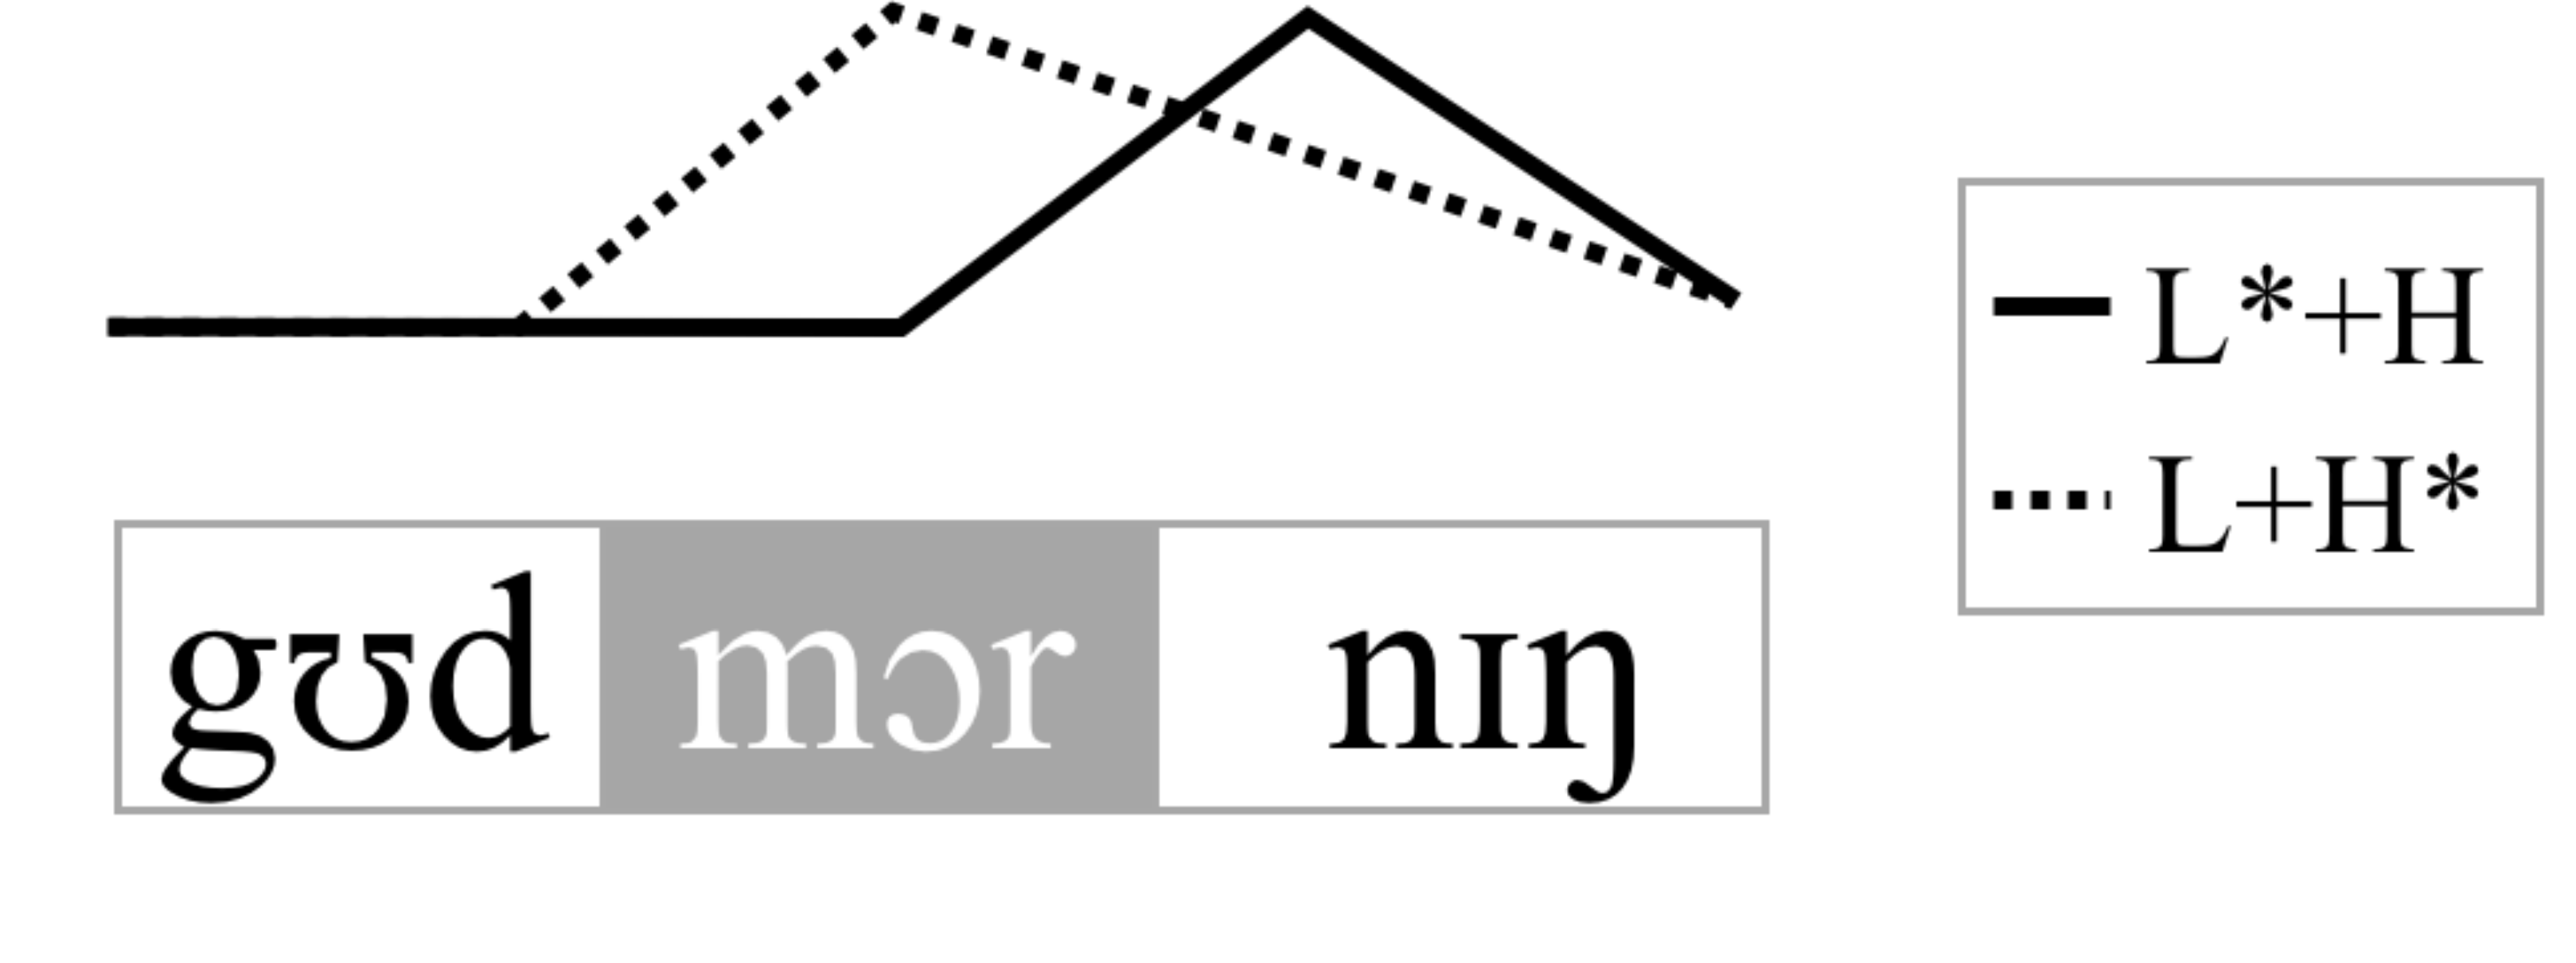
\includegraphics[width=0.6\textwidth]{figures/Figure_2_4.png}
  \caption{Schematised pitch contours for bitonal pitch accents adapted from\citet[782]{Grice2006}.} 
   \label{fig:2.4}
   \end{figure}

Later work, however, has challenged the assumption that the relationship between phonological association and phonetic alignment is that straightforward. Often, the tonal targets are phonetically instantiated close to, but not within, the TBU the tones are assumed to be associated with. \citet{Arvaniti.etal2000} demonstrated that the tonal targets of a rising pitch accent in Greek \il{Greek}do not co-occur with the accented syllable but shortly before or after it, respectively. Moreover, alignment patterns are often idiosyncratic in that they are very much dependent on the language or even the variety under investigation (e.g. \citealt{Muecke.etal2009}). \is{pitch accent}\is{tonal alignment}\is{tone bearing unit}

In addition to language-dependent factors affecting tonal alignment, there are circumstances in which the phonetic realisation of a tonal target is constrained in predictable ways. In some cases, the number of tonal targets in a tune may exceed the number of TBUs with which these tones can associate. This situation is referred to as ‘tonal crowding’. In other cases, the segmental material may be phonetically inadequate for bearing a pitch movement.\is{tonal crowding}\is{tone bearing unit}

To resolve a conflict between the need to realise functionally relevant tonal events and both the amount of TBUs available and the phonetic suitability of these TBUs, linguistic systems appear to adjust either the tones or the segments. The nature of this adjustment depends on syntagmatic, paradigmatic, as well as language-specific factors. One prominently discussed pair of notions is the distinction between ‘truncation’ and ‘compression’, both of which refer to adjustments of the realisation of tones themselves. Either a tonal target can be phonetically not reached (truncation) or the rate of pitch change between tonal targets is increased (compression). The tones can also adjust by shifting tonal targets towards less restricted segmental material. Alternatively, the tonal realisation might stay the same, while the segmental material adjusts to fulfil the requirements necessary to realise the tones. In these cases, either the segmental material may be lengthened or additional segments may be added to bear the critical tonal targets. These different strategies will be discussed in the following.\is{truncation}\is{compression}\is{tone bearing unit}\is{tonal shift}\is{vowel insertion}

\subsection{Tune-text-adjustments}\label{sec:2.4.1}
\subsubsection{Truncation and compression}
If the segmental tier offers too little sonorant material for the realisation of a tonal sequence, the f0 contour can be truncated or compressed. A useful phenomenon to shed light on truncation and compression is the lexical pitch accent contrast in Swedish\il{Swedish}: in Swedish, there are minimal pairs that are differentiated only by their lexical pitch accent (accent I and accent II). Both accent types consist of a high followed by a low target differing only in the phonetic alignment of the high tone (\citealt{Bruce1977}). In their seminal work, \citet{EriksonAlstermark1972} discuss how the realisation of a lexical pitch accent is adjusted in the face of phonotactic restrictions. On the one hand, they observed that the actual pitch movement is often reduced with decreasing vowel length, i.e. the pitch movement is undershot, with the fall after the high tone simply ending before it reaches its low target. If the syllable contains a short vowel and a voiceless coda consonant, the fall in f0 may disappear entirely. This mechanism has been named ‘truncation’. On the other hand, they discuss “rate adjustments”, where the pitch movement is realised more rapidly on shorter vowels. This mechanism has later been named ‘compression’ (\citealt{BannertBredwad1975}). \is{truncation}\is{compression}\is{tonal alignment}

\citet{Grabe1998} investigated truncation and compression  in Southern Standard British English\il{English (BE)} and Northern Standard German\il{German}. She investigated rising and falling contours phrase finally by systematically manipulating the voiced material available to realise the tonal movement, ranging from a disyllabic word with a long vowel (/ʃiːfɐ/) to a monosyllabic word with a long vowel (/ʃiːf/) to a monosyllabic word with a short vowel (/ʃɪft, ʃɪf/). Note that the stimuli contained voiceless consonants, in this way reducing the phonetic opportunity to realise tonal movements to the vowel only. Her results indicate that Southern Standard British English compresses both falls and rises. In contrast, Northern Standard German truncates falls and compresses rises. Moreover, for German, Grabe observed a gradual decrease in f0 excursion of the fall between /ʃiːfɐ/ and /ʃiːf/. For /ʃɪf/, the fall was entirely absent. This complete undershoot has also been observed in high fall-rise contours in German and Dutch \il{Dutch}(\citealt{Lickley.etal2005,Ladd2008}). In case of tonal crowding, the fall is entirely truncated resulting in a high rise. The tonal adjustment depends on the contour and the language under investigation. For example, \citet{Grabe1998} showed that f0 rises are more likely to be compressed in German and English, while the falling contour is truncated in German but compressed in English. As opposed to Grabe’s findings, \citet{Rathcke2009} showed that falling contours in German were partially compressed whereas rising–falling contours were truncated. Moreover, truncation and compression appear to be dialect dependent (\citealt{BannertBredwad1975,Grabe.etal2000}) as well as speaker specific (\citealt{PrietoOrtega2009}).\is{tonal crowding}\is{truncation}\is{compression}\is{tonal alignment}

\subsubsection{Shift of tonal targets}
A different strategy to resolve conflicts in the tune-text-association is a temporal shift of the tonal target. If there is not enough segmental material to realise a sequence of tonal targets, one or multiple tonal target may be realised earlier. A case in point is Neapolitan Italian\il{Italian (Neapolitan)}. Statements marked by a narrow focus on the final word are characterised by a local rise on the accented syllable followed by a fall within the vowel. Similarly, yes-no questions are characterised by a local rise on the accented syllable followed by a low target at the end of the utterance (\citealt{Dimperio2001}). Thus, questions and statements with final narrow focus are expressed with similar tonal events, i.e. a rise-fall in pitch phrase finally. Even though these contours appear to be very similar in certain contexts, they have been described as differing in the alignment of the high tone, which reaches its target later in the accented vowel in questions than in statements (\citealt{DimperioHouse1997}). Questions, however, can also display an additional final rise making the tonal movement very complex (a rise-fall-rise). The presence vs. absence of this final rise is dependent on dialect and speaking style (\citealt{Savino2012}). \citet{CangemiGrice2016} looked at the alignment of the high target of the pitch accent across instances with and without an utterance-final rise. They found strong evidence for the high target shifting to the left when a phrase-final rise is present. The tonal sequence starts earlier to ensure the realisation of all tonal targets. The tendency of tones to be shifted leftwards has been observed in many other languages in different contexts (\citealt{Steele1986,CaspersHeuven1993,Dimperio2001,Prieto.etal2005,Schepman.etal2006,Muecke.etal2009}).\is{tonal shift}\is{focus}\is{yes-no question}\is{tonal alignment}

\subsubsection{Adjustments of the text}
After having explored cases in which the tune adjusts to insufficient text, we now turn to adjustments of the text to the tune. The text can be adjusted in two ways: existing segmental material can be lengthened or segmental material can be added. The former case has been reported for Spanish and Catalan\il{Spanish}\il{Catalan} by \citet{PrietoOrtega2009}. They investigated the intonational marking of focus in phrase-final position. In words with final stress, narrow focus is characterised by a rise-fall on the final syllable. They compared these contours to a simpler falling contour and found that syllables are longer when the tune is more complex. This can be considered to be a mechanism to fit the complex rise-fall tonal sequence, which is not necessary for the simpler falling contour. Similar results have been reported for Bari Italian yes-no questions, which are typically realised (in read speech) with an accentual rise followed by a fall-rise. If a phrase-final accented syllable bears the rise-fall-rise, it has been found to be considerably lengthened as compared to the same syllable in neutral statements, in which there is a simple fall in the lower portion of the speaker’s range (\citealt{Grice.etal1997,Refice.etal1997}). Similarly, \citet{Frota2002} reports on lengthening of the nuclear vowel in phrase-final position when a fall-rise is to be realised in Portuguese \il{Portuguese} yes-no questions. \citet{Heston2014} reports on lengthening of utterance-final vowels when they are accompanied by a final rise-fall in Fataluku\il{Fataluku}, a Papuan language.\is{yes-no question}\is{pitch accent}\il{Italian (Bari)}

In addition to lengthening existing segments, some languages insert additional segmental material to enable tonal realisation. In Bari Italian, speakers producing loanwords ending in closed syllables often insert a schwa-like element word finally ([tɪm] vs. [tɪmə], \citealt{Grice.etal2015bari}). The presence as well as the acoustic salience of these schwas is modulated by the complexity of the tune with a greater incidence of schwa and a greater duration of schwa in more complex question tunes. Moreover, the metrical structure of the word predicts the presence and duration of schwa as well. There were more and longer schwas in monosyllabic words than in disyllabic trochaic words. This fits with the idea of schwa occurring to aid in the realisation of tones. Since a disyllabic word already contains one unaccented syllable that can carry some of the tonal complex, speakers are less likely to add an additional element. \citet{Frota2002} reports on similar insertions of non-lexical vowels in Portuguese. A high central vowel is inserted in utterances with a complex tonal movement on the final syllable.\is{vowel insertion}\il{Portuguese}

\subsubsection{Summary}
To sum up, the literature indicates different mechanisms for conflict resolution in tune-text-association. The tonal target is not reached (truncation) or the rate of pitch change is increased (compression). The tune can also adjust by shifting the tonal target towards less restricted segmental material (shift). Finally, the segmental material may be lengthened or additional segments may be added to bear the critical tonal target. These strategies are schematised in \figref{fig:2.5}.\is{vowel insertion}\is{truncation}\is{compression}\is{tonal shift}

\begin{figure}
  \centering 
   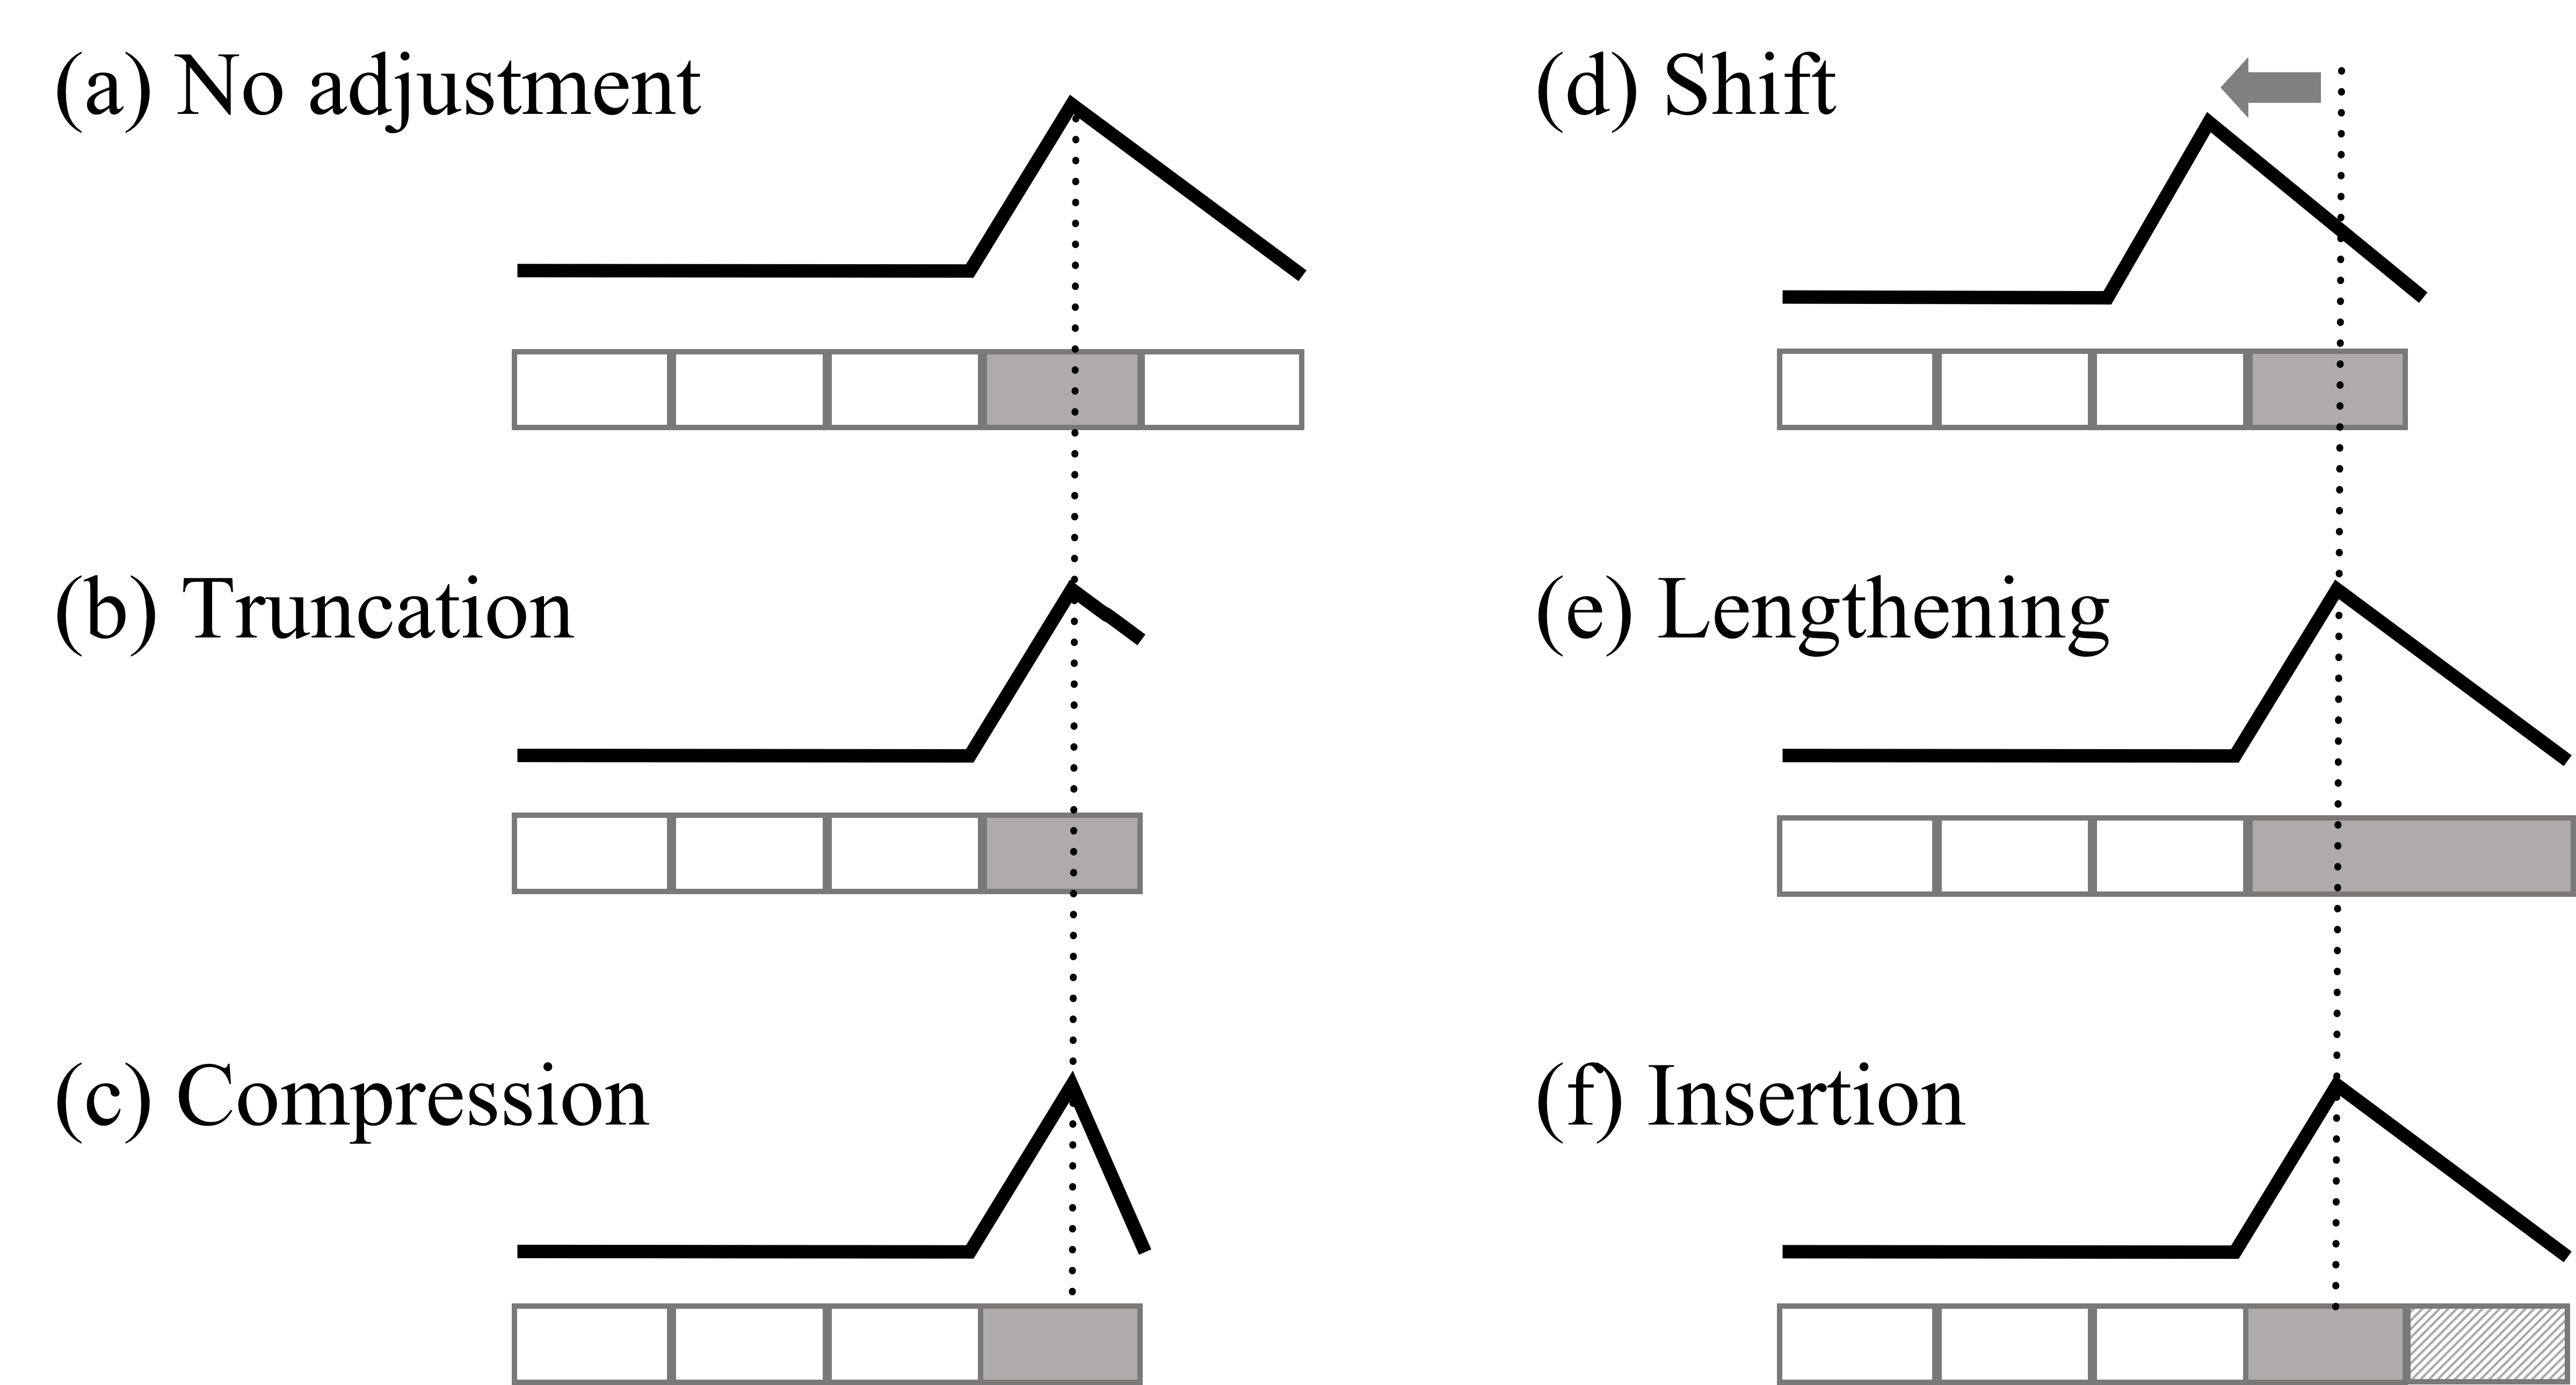
\includegraphics[width=1\textwidth]{figures/Figure_2_5.png}
  \caption{Schematic representation of tune-text-adjustments. The grey box indicates the TBU with which the rise up to a high target co-occurs. Panel (a) illustrates a case in which tune and text associate normally. The tune is characterised by a rise towards a high target on the TBU followed by a fall to a low target at the end of the utterance. In (b) the final low target is not fully reached (truncated). In (c) the rate of pitch change is compressed. In (d) the rise-fall shifts to the left. In (e) the accented syllable is lengthened. In (f) an additional segment (light grey) is added.}
   \label{fig:2.5}
   \end{figure}
   
Importantly, these strategies are not mutually exclusive. Contours can be both compressed and truncated to some degree, a shift may occur together with additional compression, and adjustments to the text may interact with adjustments to the tune. Interestingly, previous research has also demonstrated that there may be a trade-off between text-adjustment and tune-adjustments. \citet{PrietoOrtega2009} report on a negative correlation between increasing syllable duration and truncation of the contour.

\subsection{The representation of tune-text-adjustments}
Adjustments to the tune are often considered to be phonetic variants of phonologically identical contours (\citealt{Gronnum1989,Grabe1998,Grabe.etal2000,Hanssen.etal2007,Ladd2008}). One strong argument for this claim is the gradual nature of truncation. As discussed above, \citet{Grabe1998} observed a gradual decrease in f0 excursion from /ʃiːfɐ/ to /ʃiːf/ to /ʃɪf/ \il{German}which resulted in the fall being entirely absent in /ʃɪf/. Furthermore, Grabe notes that speakers hear the target words as having falling pitch regardless of the actual f0 values (\citealt[140]{Grabe1998}). This is in line with recent findings demonstrating that despite the “missing” parts of the f0 contour, the signal may bear other acoustic correlates that correspond to the intended meanings. Experiments with whispered speech have shown that noise-induced cues can be used to convey meanings that would otherwise be encoded in f0. Speakers of Mandarin compensate for the lack of F0 in whispered speech by using, for example, intensity to maintain the contrast between lexical tones (\citealt{WhalenXu1992}). The use of acoustic substitutes for f0 is not restricted to whispered speech: recent experiments have shown that in normal speech, speakers consistently make adjustments in voiceless obstruents induced by intonational contexts. In several experiments, Niebuhr and colleagues (\citealt{Niebuhr2008,Niebuhr2009,Niebuhr2012,Niebuhr.etal2011}) showed that frication and aspiration noise of phrase-medial and phrase-final voiceless obstruents corresponds to the expected modulation of f0 (see also \citealt{RitterRoettger2014}). In particular, voiceless parts of the signal corresponding to high/rising tones exhibit higher mean Centre of Gravity and higher mean intensity than counterparts of corresponding low/falling tones. Thus, even in absence of f0, the phonological representation may be phonetically manifested via other channels than f0.\is{truncation}\is{pitch scaling}\is{segmental pitch}\il{Mandarin}

While truncation in Grabe’s study appears to be gradual, other phenomena discussed in the literature have rather been regarded as discrete. In these cases, tune-text-adjustments like truncation may be interpreted as contextual variants of the unadjusted tune-text-association similar to allophony in segmental phonology. This sort of phonological account has been proposed within the AM model using the concept of ‘secondary association’.\is{truncation}\is{secondary association}

In their influential analysis of the Japanese intonation system, \citet{PierrBeck1988} proposed secondarily associated edge tones. Consider \figref{fig:2.6}. Japanese is analysed as having both lexically specified tonal events (HL on se’ and do’) and postlexical tonal events (all other tones). Syllables can be mono-moraic or bi-moraic. According to Pierrehumbert and Beckman, both the accentual phrase (α) and the utterance (υ) are delimited by edge tones. The utterance is analysed as having an initial L edge tone and a final H edge tone. The final H is considered an edge tone that is ‘primarily associated’ with the right edge of the utterance. The initial L tone is −in addition to being primarily associated with the left edge of the utterance− also associated with a tone bearing unit, the first sonorant mora in the utterance. \is{secondary association}\is{edge tone}\is{tone bearing unit} \il{Japanese}

\begin{figure}
  \centering 
   
\includegraphics[width=0.8\textwidth]{figures/Figure_2_6.png}
  \caption{Pierrehumbert and Beckman’s analysis of prosodic structure and tonal association for following Japanese sentence: Ane-no akai se’etaa-wa do’ko desu ka? (‘Where is big sister’s red sweater?’, adapted from \citet[21]{PierrBeck1988}). Dashed line indicates secondary association to a TBU.}
   \label{fig:2.6}
   \end{figure}
   
Similarly, accentual phrases have a left H edge tone and a right L edge tone. Both tones are conceived of as secondarily associated with a sonorant mora. The accentual phrase-initial H tone associates with the second mora, because the higher-level utterance-initial edge tone is associated with the first mora. The accentual phrase-final edge tone, the L, is analysed as secondarily associated with the first mora of the following accentual phrase, pushing the accentual phrase-initial edge tone to the second mora. Note that in this analysis not all edge tones are secondarily associated. For example, the final L edge tone of the second accentual phrase is only primarily associated with the edge and has no secondary association.\is{secondary association}\is{edge tone}
 
\newpage  
The accentual phrase-final L tone (indicated by superscripted a) is realised on the first mora of the upcoming accentual phrase if two conditions are met: the first syllable in the phrase must be mono-moraic and unaccented (i.e. here, it does not bear the HL). This results in an association of the accentual phrase-initial H tone (indicated by superscripted b) to the second mora (as in akaise’e taa wa, \figref{fig:2.6}).

There are two scenarios in which the first mora of the accentual phrase is not associated with the L tone but instead with a H tone: either the first syllable is bi-moraic in which case phrase-initial H is associated to the first mora (not in \figref{fig:2.6}), or the first syllable is accented (bearing the HL, indicated by superscripted c). When the first mora bears a H tone, the L tone realisation is reported to be “phonetically weak”, i.e. the pitch is not as low, the rise to the H is shorter and flatter or it is entirely absent. In cases with a short unaccented first mora, the L tone preceding the H is realised as “phonetically strong”, i.e. there is a clear rise from low to high pitch. 

\newpage 
This analysis attempted to account for the distributional properties of intonational tones in \il{Japanese}Japanese. The difference in the phonetic realisation of the proposed tones is accounted for by two different phonological association patterns, and in turn, with two different categories of edge tones: an edge tone that has only a primary association and an edge tone that has an additional secondary association to a tone bearing unit.\is{secondary association}\is{edge tone}\is{tone bearing unit}\is{tonal association}

\citet{Grice1995} has applied this theoretical concept to Palermo Italian question intonation. Yes-no questions in the Palermo variety are produced with a rise-fall in pitch consisting of a rising pitch accent (L+H* in Grice’s annotation) and low edge tone (L-). When the final syllable is accented, the subsequent fall does not fully reach a low target. However, if the accented syllable is not final, there is a deep fall towards a full low pitch target. This resembles the truncation phenomena described in \sectref{sec:2.4.1}. As opposed to \citet{Grabe1998}, however, Grice accounts for this difference by means of phonological association patterns. In the case of a final accent, the low edge tone is primarily associated to the edge. In the case of a non-final accent, the edge tone is secondarily associated to the final syllable making it lower in pitch. One argument for this analysis put forward by Grice is the rather discrete nature of this alternation in terms of both distributional observations and auditory impressions.\is{secondary association}\is{edge tone}\is{yes-no question}\is{pitch accent}\is{truncation}\is{tonal association}\il{Italian (Palermo)}

Gussenhoven applied a similar analysis to tonal phenomena in Venlo Dutch accounting for the alignment properties of low edge tones (\citealt{GussenhovenVanderVliet1999,Gussenhoven2000,Gussenhoven2002}). After a high pitch accent marking focus, the low edge tone can be aligned right after the high target, resulting in a sharp fall, or at the edge, resulting in a slow fall towards the phrase edge. If the stressed syllable is bi-moraic, the fall occurs right after the high target of the pitch accent and the high pitch accent is analysed as associating with the first mora of the stressed syllable. Alternatively, if the stressed syllable is mono-moraic, there is a late, imprecise fall towards the end of the phrase. Gussenhoven accounted for this asymmetry by proposing a secondary association of the low edge tone to the second mora of the accented syllable. If not available, the low edge tone remains primarily associated to the boundary with no secondary association.\is{secondary association}\is{tonal alignment}\is{focus}\is{edge tone}\is{pitch accent}\il{Dutch (Venlo)}

  
Whether tune-text-adjustments, as discussed in the previous section, are adjustments of the phonetic realisations, leaving the phonological representation unchanged, or a phonetic reflex of a phonological alternation, remains an empirical question to be answered for each language individually. While the gradual nature of truncation in Grabe’s study (\citeyear{Grabe1998}) indicates a non-phonological nature of tune-text-adjustments in German, \citeauthor{Grice1995}’s reports on Palermo Italian (1995) suggest a representational difference. Such cases can be seen as context-dependent allophonic alternations paralleling to context-dependent alternations in the segmental domain. Secondary association can be conceived of as a way to formalise such context-dependent allophonic alternations and, in turn, enables an allocation of tune-text-adjustments to the level of phonological representation. \is{secondary association}\is{truncation}\il{Italian (Palermo)}

The concept of secondary association was substantially extended and made more explicit in \citet{Grice.etal2000}. They used this formal mechanism to account for phonological differences of a particular tune across varieties of Hungarian, Romanian, and Greek\il{Hungarian}\il{Romanian}\il{Greek}: ‘the Eastern European question tune’ (EEQT). All of these languages express yes-no questions with a similar intonation contour, characterised by a rise-fall. In all investigated languages, the contour can be analysed as having a low nuclear pitch accent on the stressed syllable of the accented word (L*), a rise to a high tone (H), and a fall to a low tone at the right edge of the phrase (L\%). However, they differ with regard to the position of the H tone. The H tone occurs either on the stressed syllable in a word occurring after the accented word or on a specific syllable close to the right edge of the phrase (dependent on the position of the accented word and the language under investigation). Take for example Standard Greek\il{Greek}. When the nuclear accent (L*) is on a non-final word, the H phrase accent (H-) is secondarily associated with the lexically stressed syllable of the final word (\figref{fig:2.7}a). If the nuclear accent is on the final word, the H phrase accent is secondarily associated with the final syllable (\figref{fig:2.7}b). Grice et al. account for these contours by proposing a phrase edge tone (H-) that is secondarily associated to a particular syllable (post-nuclear stressed syllable or a syllable close to the phrase edge). Given this analysis, the languages investigated by Grice et al. share the same phonological representation differing only in the unit with which the H tone is secondarily associated. They refer to this tone as a ‘phrase accent’ and define it as an edge tone with the possibility of a secondary association to a tone bearing unit. These tones, even though clearly not signalling prominence or focus, share some of the properties of pitch accents when they are associated with a TBU such as enhancing the spatio-temporal aspects of the segments with which they co-occur. So phrase accents are argued to be at once edge tones (‘phrase-’) and prominence lending tones (‘-accent’). \is{secondary association}\is{yes-no question}\is{phrase accent}\is{pitch accent}\is{edge tone}\is{focus}

\begin{figure}
  \centering 
   
\includegraphics[width=1\textwidth]{figures/Figure_2_7.png}
  \caption{The East European Question Tune for Standard Greek analysed as phrase accents that are secondarily associated with the text (according to \citealt{Grice.etal2000}).} 
   \label{fig:2.7}
   \end{figure}

\section{Summary}\label{sec:2.5}
The present chapter has introduced relevant concepts of intonation and prosodic structure. These notions were elaborated on within the Autosegmental-Metrical model (AM). The AM model is characterised by two assumptions. It assumes that sounds are grouped into hierarchically organised sets of constituents and it proposes separate levels of description for segments and tonal events. These levels are associated with each other. Based on these assumptions, certain key phenomena of intonation were discussed. Tonal events are defined by properties of their phonetic form such as their temporal alignment with the segmental material as well as by the function they express. Edge tones are phonologically associated with the edges of prosodic constituents. Pitch accents are phonologically associated with designated terminal elements of prosodic constituents. These designated terminal elements usually coincide with the stressed syllable of a word. Since the notion of pitch accent presupposes the presence of metrical prominence asymmetries at the word level, it is limited with regard to its applicability. Languages without word stress cannot be described as having a pitch accent in the sense used here, namely a postlexical tone or tonal complex associated with a lexically determined strong syllable.

With regard to functional differences, edge tones are commonly described as marking edges and signalling communicative functions such as sentence modality (questions vs. statement) and (non-)finality. Pitch accents are commonly described as marking prominent elements of the phrase such as new and contrastive information. 

In addition to edge tones and pitch accents, certain tones fall in neither category: some of these tonal events can be captured by the concept of the phrase accent. Phrase accents associate to the edge, but do not have to be aligned to it. They can appear on a TBU near the edge, either a stressed syllable or an unstressed syllable that is close to the edge. They do not signal focus, but appear to have prominence-lending qualities. The introduction of the phrase accent constitutes a development in intonation research (and the AM model) that demonstrates the fruitfulness of decomposing typological categories into their distributional and functional characteristics. 

It becomes clear that the association of the tune and the text is one crucial criterion for categorising tonal events. This association, however, is not always straightforward. In certain contexts, the phonetic realisation of a tonal event is restricted, either due to crowding of tones or due to the segmental identity of the TBU. Facing such conflicts, linguistic systems adjust either the tones or the segmental material by truncating or compressing the contour, shifting the tonal target, lengthening the available segmental material, or inserting additional segments. Both the choice of strategy as well as its linguistic status depend on the language under investigation and the analysis. Some phenomena exhibit gradual and predictable properties; others appear to be best captured by assigning them (allo-)phonological status.

While most work on tune-text-association has been done on languages in which well-formed syllables usually contain at least a sonorant, work on tune-text-association in languages with more extreme phonotactic possibilities is rare. There are languages that allow whole utterances without phonological vowels and words that are comprised of voiceless segments only. In these cases, the phonetic opportunity for the execution of intonational pitch movements is constrained. The question arises as to how the tune associates with the text in these cases. Here, we will attempt to answer this question by studying intonation in Tashlhiyt, a Berber language.

